% Options for packages loaded elsewhere
\PassOptionsToPackage{unicode}{hyperref}
\PassOptionsToPackage{hyphens}{url}
%
\documentclass[
]{book}
\usepackage{amsmath,amssymb}
\usepackage{lmodern}
\usepackage{ifxetex,ifluatex}
\ifnum 0\ifxetex 1\fi\ifluatex 1\fi=0 % if pdftex
  \usepackage[T1]{fontenc}
  \usepackage[utf8]{inputenc}
  \usepackage{textcomp} % provide euro and other symbols
\else % if luatex or xetex
  \usepackage{unicode-math}
  \defaultfontfeatures{Scale=MatchLowercase}
  \defaultfontfeatures[\rmfamily]{Ligatures=TeX,Scale=1}
\fi
% Use upquote if available, for straight quotes in verbatim environments
\IfFileExists{upquote.sty}{\usepackage{upquote}}{}
\IfFileExists{microtype.sty}{% use microtype if available
  \usepackage[]{microtype}
  \UseMicrotypeSet[protrusion]{basicmath} % disable protrusion for tt fonts
}{}
\makeatletter
\@ifundefined{KOMAClassName}{% if non-KOMA class
  \IfFileExists{parskip.sty}{%
    \usepackage{parskip}
  }{% else
    \setlength{\parindent}{0pt}
    \setlength{\parskip}{6pt plus 2pt minus 1pt}}
}{% if KOMA class
  \KOMAoptions{parskip=half}}
\makeatother
\usepackage{xcolor}
\IfFileExists{xurl.sty}{\usepackage{xurl}}{} % add URL line breaks if available
\IfFileExists{bookmark.sty}{\usepackage{bookmark}}{\usepackage{hyperref}}
\hypersetup{
  pdftitle={Modelado y Análisis Espacial},
  pdfauthor={Gerardo Martín},
  hidelinks,
  pdfcreator={LaTeX via pandoc}}
\urlstyle{same} % disable monospaced font for URLs
\usepackage{longtable,booktabs,array}
\usepackage{calc} % for calculating minipage widths
% Correct order of tables after \paragraph or \subparagraph
\usepackage{etoolbox}
\makeatletter
\patchcmd\longtable{\par}{\if@noskipsec\mbox{}\fi\par}{}{}
\makeatother
% Allow footnotes in longtable head/foot
\IfFileExists{footnotehyper.sty}{\usepackage{footnotehyper}}{\usepackage{footnote}}
\makesavenoteenv{longtable}
\usepackage{graphicx}
\makeatletter
\def\maxwidth{\ifdim\Gin@nat@width>\linewidth\linewidth\else\Gin@nat@width\fi}
\def\maxheight{\ifdim\Gin@nat@height>\textheight\textheight\else\Gin@nat@height\fi}
\makeatother
% Scale images if necessary, so that they will not overflow the page
% margins by default, and it is still possible to overwrite the defaults
% using explicit options in \includegraphics[width, height, ...]{}
\setkeys{Gin}{width=\maxwidth,height=\maxheight,keepaspectratio}
% Set default figure placement to htbp
\makeatletter
\def\fps@figure{htbp}
\makeatother
\setlength{\emergencystretch}{3em} % prevent overfull lines
\providecommand{\tightlist}{%
  \setlength{\itemsep}{0pt}\setlength{\parskip}{0pt}}
\setcounter{secnumdepth}{5}
\usepackage{booktabs}
\ifluatex
  \usepackage{selnolig}  % disable illegal ligatures
\fi
\usepackage[]{natbib}
\bibliographystyle{apalike}

\title{Modelado y Análisis Espacial}
\author{Gerardo Martín}
\date{2022-01-19}

\begin{document}
\maketitle

{
\setcounter{tocdepth}{1}
\tableofcontents
}
\hypertarget{preuxe1mbulo}{%
\chapter{Preámbulo}\label{preuxe1mbulo}}

\begin{center}
\includegraphics[width=6.03in]{logo} \end{center}

En el curso \textbf{Modelado y Análisis Espacial} aprenderemos a utilizar algunas herramientas para aprender a usar herramientas geográficas para analizar y representar procesos ambientales en el espacio. Los contenidos del índice se apegan al \href{Programa-curso.pdf}{programa completo del curso}, el cual se impartirá en los \href{Horario.pdf}{horarios normales establecidos}. Para conocer cuándo, cómo y qué temas se se impartirán puedes consultar la \href{Estrategia-docente.pdf}{estrategia docente}.

\hypertarget{encuadre-de-la-materia}{%
\chapter{Encuadre de la materia}\label{encuadre-de-la-materia}}

\hypertarget{criterios-de-evaluaciuxf3n}{%
\section{Criterios de evaluación}\label{criterios-de-evaluaciuxf3n}}

Las constribuciones a cada calificación parcial serán:

\begin{itemize}
\tightlist
\item
  Asistencia (25\%)
\item
  Trabajos de clase cumplidos (50\%)
\item
  Examen (25\%)
\item
  Participación (2 puntos extra máximo)
\end{itemize}

Cabe señalar, que la asistencia no corresponderá con su presencia en las sesiones sincrónicas, sino con el cumplimiento de los trabajos de clase. La participación se medirá tanto por participación directa en las sesiones sincrónicas como por el seguimiento que uds den a la clase por correo electrónico.

\hypertarget{cuxf3mo-se-daruxe1n-las-clases}{%
\section{¿Cómo se darán las clases?}\label{cuxf3mo-se-daruxe1n-las-clases}}

Trataré de apegarnos a los tiempos de actividades sincrónicas y asincrónicas establecidos en la \href{Estrategia-docente.pdf}{estrategia docente}, pero éstos son completamente flexibles. Una estrategia que me ha funcionado en cursos anteriores ha sido la de dedicar la última actividad sicrónica de la semana a resolver dudas, es en estas sesiones en las que hay muchas posibilidades de conseguir puntos de participación.

Todos los contenidos del curso, lecturas y presentaciones, se irán añadiendo a este sitio web conforme avanza el semestre. En el Google Classroom de la materia se irán anunciando las diferentes actividades y sesiones sincrónicas con anticipación suficiente. Igualmente, los examenes y resultados serán publicados a través de esta plataforma. A petición de uds, también se publicarán aquí los videos de las sesiones sincrónicas que tengamos, en especial para aquellos temas que sean mayor interés/dificultad/importancia. Los trabajos de práctica también se publicarán en Classroom.

Para finalizar, las clases sincrónicas estarán almacenadas en la playlist de la clase contenida en mi canal de youtube.

\hypertarget{reglas-del-saluxf3n}{%
\section{Reglas del salón}\label{reglas-del-saluxf3n}}

Estas, obviamente, son particulares del modelo en línea, por lo tanto aquí van las reglas de zoom:

\begin{enumerate}
\def\labelenumi{\arabic{enumi}.}
\tightlist
\item
  Micrófonos apagados
\item
  Cámaras prendidas, exceptuando:
  2.1. Si su velocidad de internet lo dificulta
  2.2. Si tienen datos limitados
\item
  Hacer muchas preguntas
\item
  Decirme si paso algo por alto
\end{enumerate}

\hypertarget{contacto}{%
\section{Contacto}\label{contacto}}

Para reportar fallos, resolver dudas y peticiones especiales grupales o individuales por favor enviar correo electrónico a \href{mailto:gerardo.mmc@enesmerida.unam.mx}{\nolinkurl{gerardo.mmc@enesmerida.unam.mx}}.

\hypertarget{unidad-i-introducciuxf3n-al-modelado-espacial}{%
\chapter{Unidad I: Introducción al modelado espacial}\label{unidad-i-introducciuxf3n-al-modelado-espacial}}

\hypertarget{anuxe1lisis-utilizando-sistemas-de-informaciuxf3n-geogruxe1fica}{%
\section{Análisis utilizando sistemas de información geográfica}\label{anuxe1lisis-utilizando-sistemas-de-informaciuxf3n-geogruxe1fica}}

\hypertarget{introducciuxf3n}{%
\subsection{Introducción}\label{introducciuxf3n}}

En el mundo moderno hay una gran cantidad de procesos y servicios que utilizan información espacial. Más allá de las aplicaciones comerciales que ya todxs conocemos hoy por hoy, los sistemas de información geográficas (SIG) son altamente necesarios para planear muchas de las actividades de las sociedades, por ejemplo para identificar áreas:

\begin{itemize}
\tightlist
\item
  donde se permitirá la urbanización
\item
  prioritarias de conservación
\item
  donde se puede practicar la agricultura
\item
  donde se puede producir energías renovables
\item
  que se pueden ver afectadas por desastres naturales
\end{itemize}

Además de identificación de zonas relevantes, también sirven para la cuantificación tanto de superficies como de poblaciones humanas. En ciencas ambientales, nos interesaría aprender a utilizar los SIG para solventar problemáticas ambientales sobretodo aquellas resultado de las actividades del ser humano. Las soluciones ambientales requieren tanto de la identificación espacial como del monitoreo, manejo y mitigación, cuyo éxito puede depender en gran medida de la disponibilidad de información geográfica.

\hypertarget{ejercicio}{%
\subsection{Ejercicio}\label{ejercicio}}

Visita la página del \href{https://sedac.ciesin.columbia.edu/}{Socioeconomic Data and Applications Center} y navega por los diferentes apartados temáticos que cubren, haciendo una lista con descripciones de mapas que te parezcan interesantes o relevantes.

\hypertarget{quuxe9-son-los-sig}{%
\subsection{¿Qué son los SIG?}\label{quuxe9-son-los-sig}}

Los SIG son programas de computadora especializados en el manejo, análisis y visualización de datos geográficos. Estos últimos a grandes rasgos con una descripción numerica o cualitativa que esté georreferenciada, o bien, que represente la forma o algún atributo de un objeto cuya localización se conoce. Los sistemas de información geográfica por lo general utilizan distintos tipo de datos.

\hypertarget{imuxe1genes-ruxe1ster}{%
\subsubsection{Imágenes ráster}\label{imuxe1genes-ruxe1ster}}

Consisten de píxeles que representan valores con alguna paleta de colores

\begin{figure}

{\centering 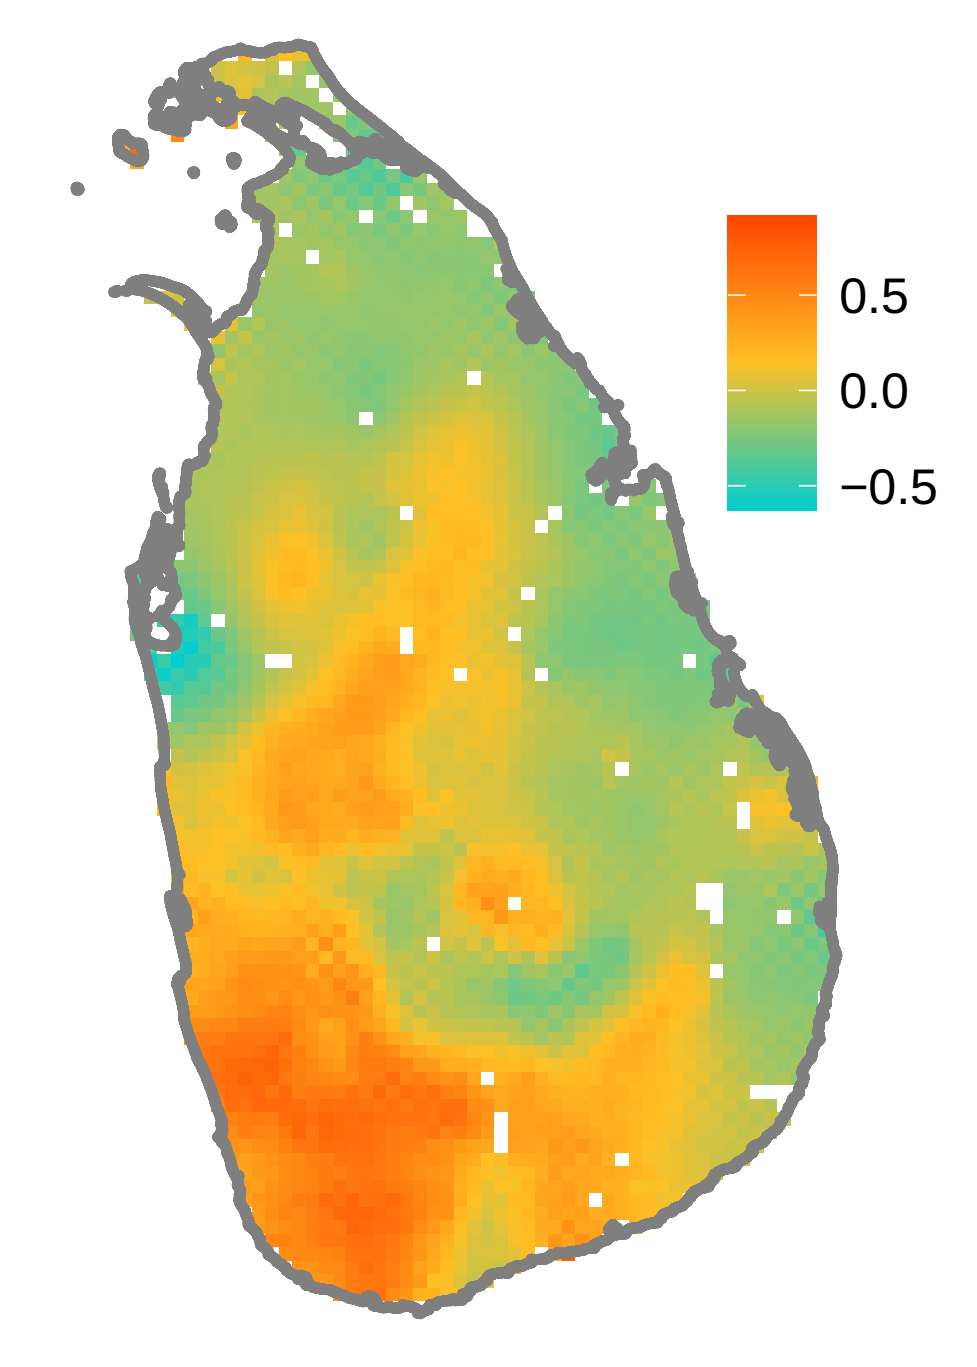
\includegraphics[width=13.57in]{Unidad-I/Rho-snakebites} 

}

\caption{Ejemplo de capa ráster de algún atributo ambiental de la isla de Sri Lanka. Cada píxel mide 5 x 5 km.}\label{fig:unnamed-chunk-5}
\end{figure}

\hypertarget{capas-vectoriales}{%
\subsubsection{Capas vectoriales}\label{capas-vectoriales}}

Pueden representar tanto polígonos como líneas. Los polígonos son utilizados para representar entidades políticas como los países o estados. Las capas vectoriales de líneas pueden utilizarse para representar ríos o caminos

\begin{verbatim}
## OGR data source with driver: ESRI Shapefile 
## Source: "/home/gerardo/Documentos/Cosas ENES/Materias/LCA/Analisis-Modelado-Espacial/Unidad-I/SL-1/LKA_adm1.shp", layer: "LKA_adm1"
## with 25 features
## It has 14 fields
## Integer64 fields read as strings:  ID_0 ID_1 CCN_1
\end{verbatim}

\begin{figure}

{\centering 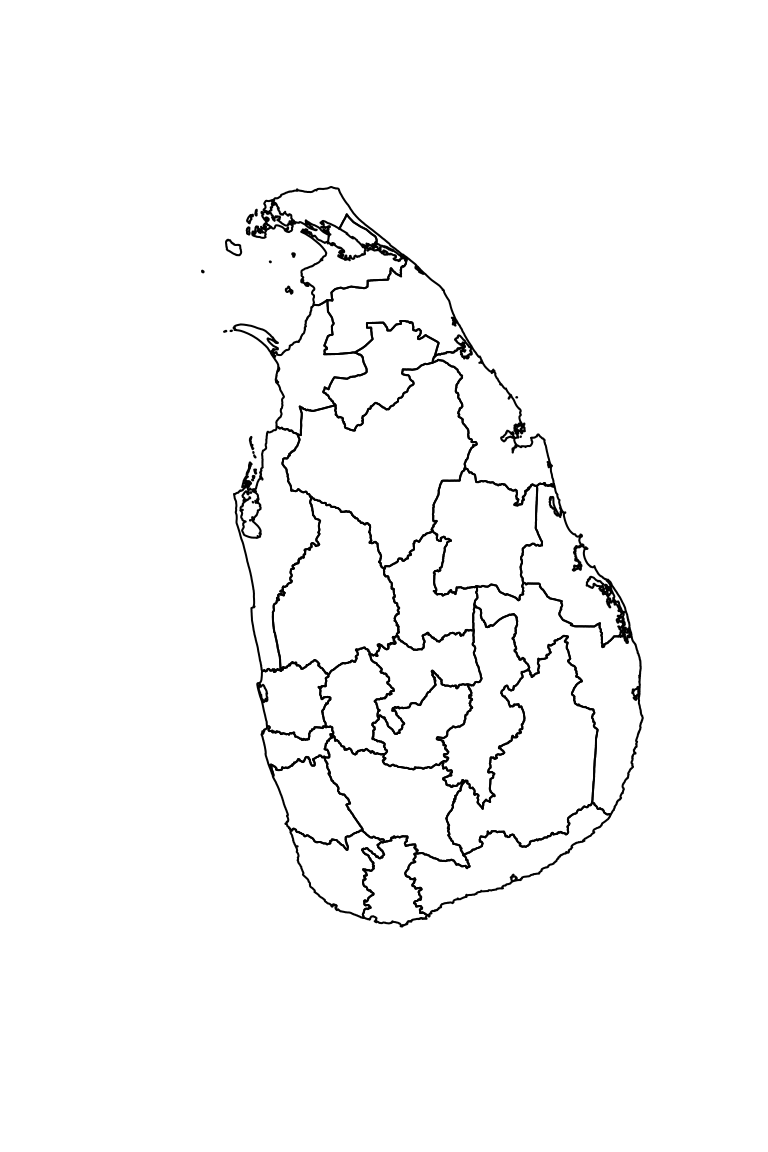
\includegraphics{Mod-mat-ECO_files/figure-latex/unnamed-chunk-6-1} 

}

\caption{Polígono vectorial muestra la isla de Sri Lanka y su división política en distritos.}\label{fig:unnamed-chunk-6}
\end{figure}

\begin{verbatim}
## OGR data source with driver: ESRI Shapefile 
## Source: "/home/gerardo/Documentos/Cosas ENES/Materias/LCA/Analisis-Modelado-Espacial/Unidad-I/Roads/LKA_roads.shp", layer: "LKA_roads"
## with 500 features
## It has 5 fields
\end{verbatim}

\begin{figure}

{\centering 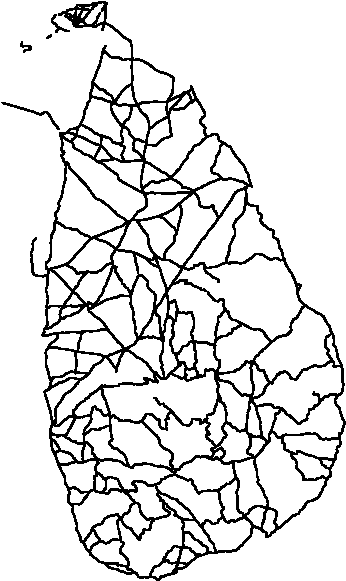
\includegraphics{Mod-mat-ECO_files/figure-latex/unnamed-chunk-7-1} 

}

\caption{Capa lineal muestra la red de carreteras principales de la isla de Sri Lanka.}\label{fig:unnamed-chunk-7}
\end{figure}

\hypertarget{puntos}{%
\subsubsection{Puntos}\label{puntos}}

Son conjuntos de coordenadas geográficas (\(x, y\)) cartesianas para identificar la localización de un objeto en el espacio.

\begin{figure}

{\centering 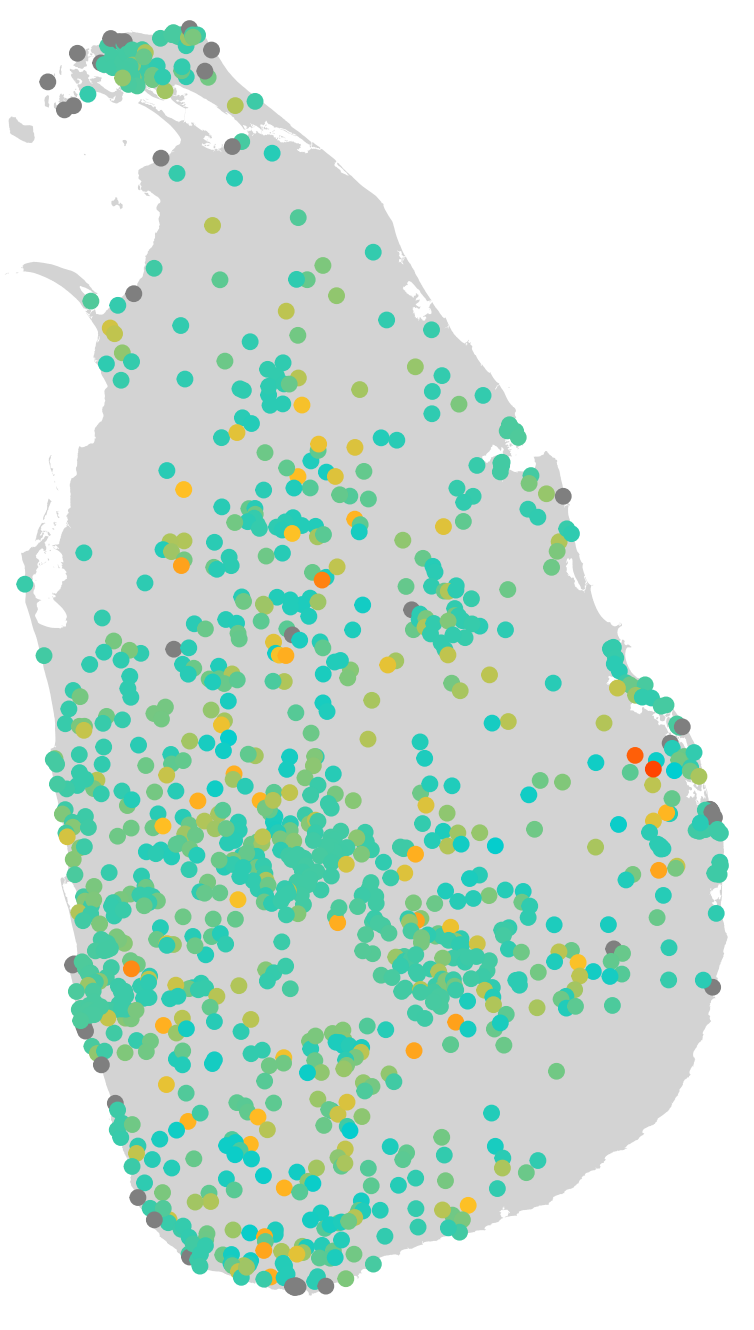
\includegraphics[width=10.47in]{Unidad-I/Survey-residuals-snakebites} 

}

\caption{Puntos muestran el valor de una medición de alguna variable ambiental en la isla de Sri Lanka.}\label{fig:unnamed-chunk-8}
\end{figure}

\hypertarget{ejercicio-1}{%
\subsubsection{Ejercicio}\label{ejercicio-1}}

Vuelve a visitar el \href{https://sedac.ciesin.columbia.edu/}{Socioeconomic Data and Applications Center} y clasifica los mapas que seleccionaste anteriormente de acuerdo con el tipo de datos que consideres que contiene cada uno.

\hypertarget{cuxf3mo-puedo-conseguir-un-sig}{%
\subsection{¿Cómo puedo conseguir un SIG?}\label{cuxf3mo-puedo-conseguir-un-sig}}

Al igual que con los sistemas operativos (Windows, Mac) y las suites de ofimática (Google Docs, MS Office, Libre Office), existen alternativas tanto comerciales (de pago y código cerrado) como libres (tanto de pago --gratis-- como de código fuente). Uno de los SIG más completos que existen es ArcGIS, sin embargo costo de la licencia es bastante alto. PAra evitar la necesidad de pagar licencias, en este curso, utilizaremos QGIS (Quantum GIS), Saga y R, pues son gratuitos y cubren todas las necesidades del curso y muchas más. De hecho, estas herramientas son sumamente competentes tanto para estudiantes como para profesionales que requieren de aplicaciones sofisticadas, por lo que la relación costo-beneficio es insuperable.

Para instalar QGIS visita la \href{https://qgis.org/es/site/}{página web} y sigue las instrucciones de instalación para tu sistema operativo. Los demás programas los instalaremos en otra ocasión.

\hypertarget{modelado-espacial}{%
\section{Modelado espacial}\label{modelado-espacial}}

El modelado y análisis espacial puede ser tan variado como los tipos de datos y variables que se pueden representar en el espacio.

Es posible modelar datos vectoriales, puntos y hasta ráster.

\hypertarget{datos-vectoriales}{%
\subsection{Datos vectoriales}\label{datos-vectoriales}}

Ejemplos clásicos abundan en la literatura médica, donde típicamente se analiza el número de casos por polígono de alguna enfermedad.

\begin{figure}
\centering
\includegraphics{https://www.multibugs.org/documentation/latest/spatial/maps2.bmp}
\caption{Casos de cancer labial en Escocia}
\end{figure}

\hypertarget{ruxe1ster}{%
\subsection{Ráster}\label{ruxe1ster}}

El típico análisis de imágenes ráster es el desarrollo de mapas de uso de suelo. Sin embargo existen otras aplicaciones como la estimación de densidad poblacional de humanos a partir de imágenes satelitales.

\begin{figure}
\centering
\includegraphics{https://www.worldpop.org/img/methods2/populations/thumbnail_peanutButter_overview3.jpg}
\caption{Estimación de densidad poblacional combinando imágenes satelitales y vectoriales}
\end{figure}

\hypertarget{unidad-ii}{%
\chapter{Unidad II}\label{unidad-ii}}

\hypertarget{unidad-iii}{%
\chapter{Unidad III}\label{unidad-iii}}

\hypertarget{unidad-iv}{%
\chapter{Unidad IV}\label{unidad-iv}}

\hypertarget{unidad-v}{%
\chapter{Unidad V}\label{unidad-v}}

\hypertarget{unidad-vi}{%
\chapter{Unidad VI}\label{unidad-vi}}

  \bibliography{book.bib,packages.bib,citas.bib}

\end{document}
